% !TEX root = ../main.tex
\begin{document}

\section{ソフトウェアテストの結果について}
入力内容と期待される出力内容を表\ref{入力内容と期待される出力内容}に示す。
\begin{table}[H]
    \centering
    \caption{入力内容と期待される出力内容}
    \label{入力内容と期待される出力内容}
\end{table}
\begin{longtable}{|c|c|c|c|} % \hline
    \hline
    入力内容 & 期待される出力内容(例) & 実際の出力内容 & 期待される結果と実際の結果の比較 \\ \hline
    \endfirsthead
    \hline
    入力内容 & 期待される出力内容(例) & 実際の出力内容 & 期待される結果と実際の結果の比較 \\ \hline
    \endhead
    % \hline
    \endfoot
    1 & 4.000000 & 4.000000 & 正しく動作している \\
    10 & 3.600000 & 3.600000 & 正しく動作している \\
    100 & 2.840000 & 2.840000 & 正しく動作している \\
    1000 & 3.168000 & 3.168000 & 正しく動作している \\
    10000 & 3.149600 & 3.149600 & 正しく動作している \\
    100000 & 3.138520 & 3.138520 & 正しく動作している \\
    1000000 & 3.142096 & 3.142096 & 正しく動作している \\
    10000000 & 3.141878 & 3.141878 & 正しく動作している \\
    100000000 & 3.141438 & 3.141438 & 正しく動作している \\
    1000000000 & 3.141588 & 3.141588 & 正しく動作している \\
    \hline
\end{longtable}
入力する値が大きくなるに連れて、おおよそ実際の出力も円周率に近くなっていることから、プログラムは正しく動作している。

以下にプログラムの実行結果を示す。

\begin{figure}[H]
    \centering
    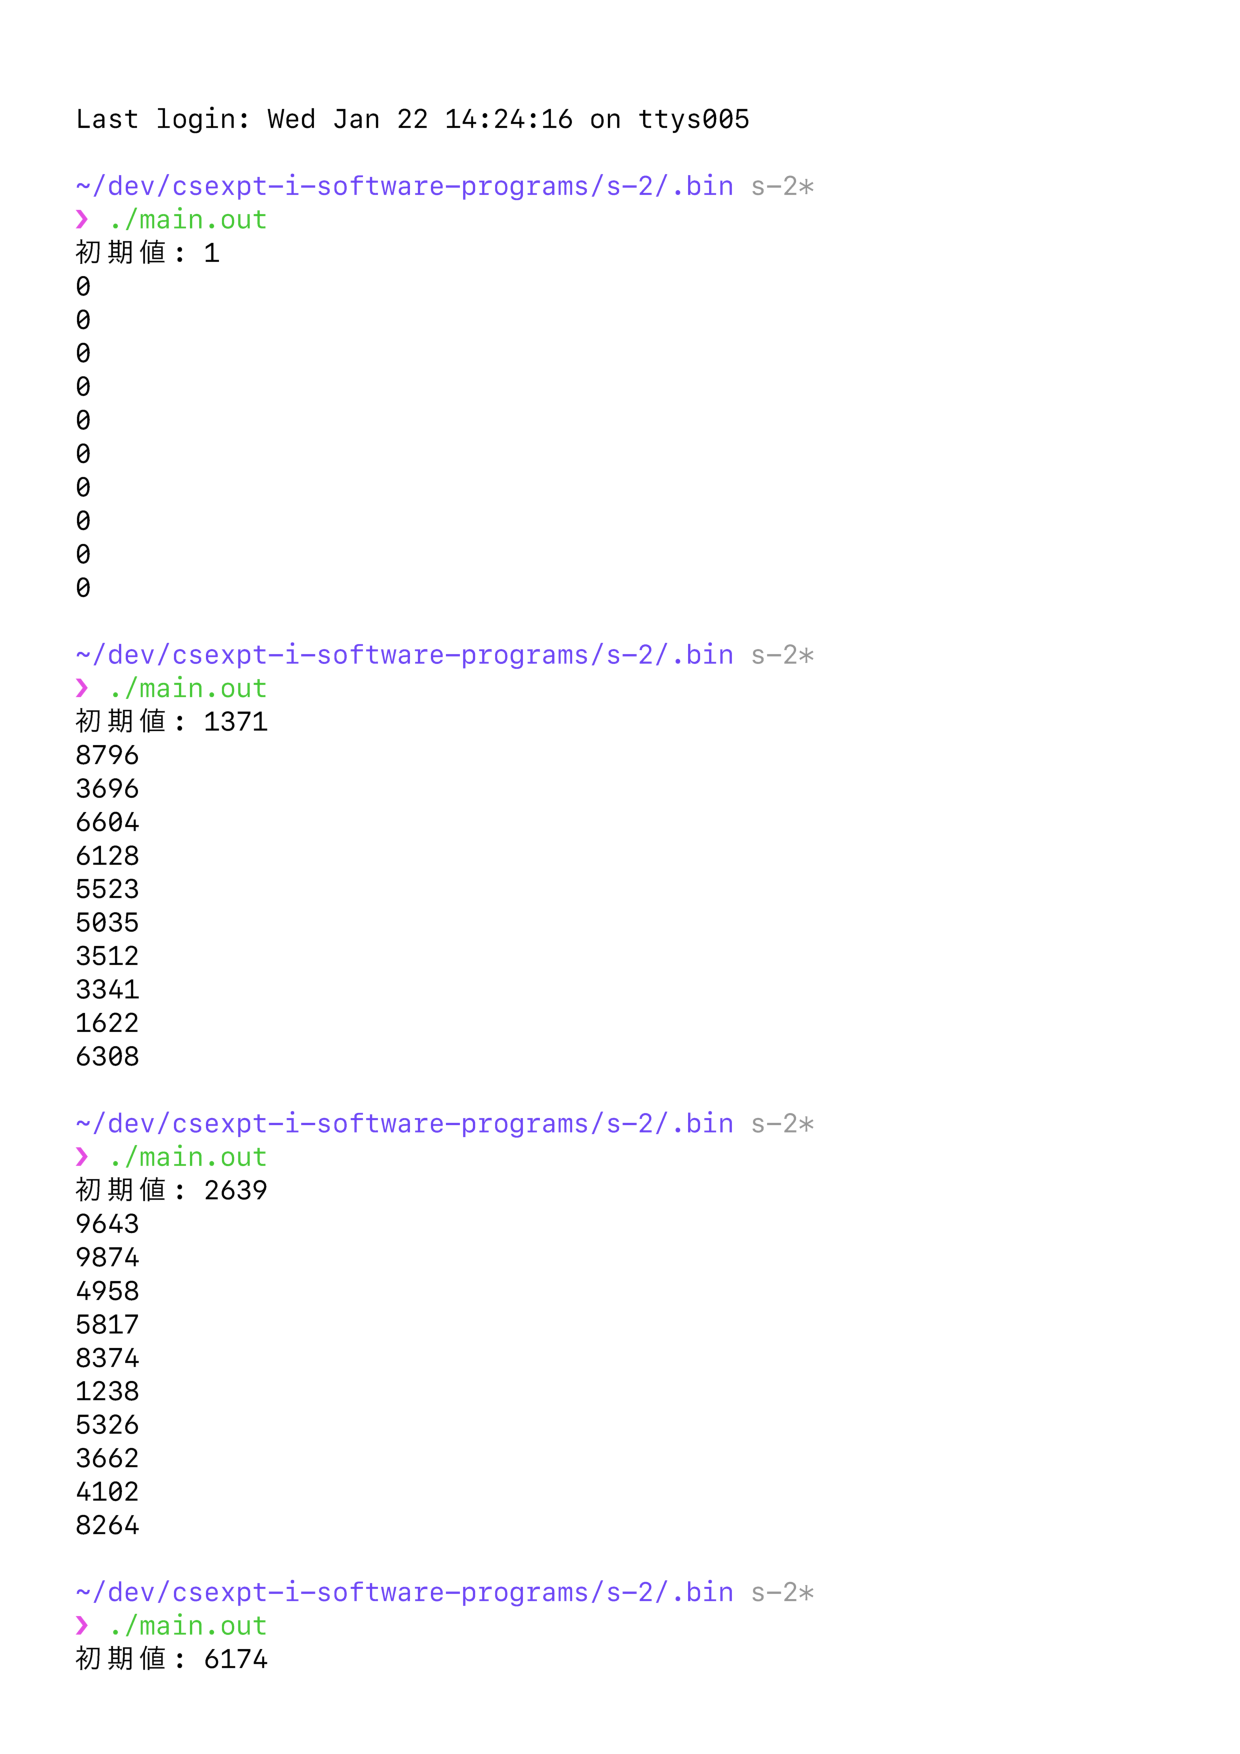
\includegraphics[width=0.8\hsize, pagebox=mediabox, page=1]{main_result_img.pdf}
    \caption{実行結果}
    \label{実行結果}
\end{figure}

表\ref{入力内容と期待される出力内容}の結果より、期待された出力を行っているから、プログラムリスト\ref{作成したプログラム}は正しい。

\end{document}
